\chapter{Calibrating the Sexual Contacts Network }\label{Calibrado}

The calibration of this kind of random computational models is an open problem and several issues about fitting computational models to data with uncertainty have to be addressed. For instance, 

\begin{itemize}
	\item the fact that, for the same set of parameters, different realizations usually return different outputs, and consequently, one realization may fulfill the fitting requirements and another realization does not,
	\item the determination of an appropriate measure of goodness-of-fit,
	\item to find model parameters agreeing the values appearing in the medical literature in a reliable and reproducible way,
	\item adaptation of the optimization algorithms to these above issues and the available resources,
	\item the determination of the best parallel implementation of the optimization algorithms, in terms of quality of the solutions and computational efficiency of the program.
\end{itemize} 

In the remainder of this section, we are going to describe thoroughly the procedure we propose to approach the above issues.

\section{Description of the model}\label{sec:modelo}
As we explained in Chapter \ref{ConstruccionYDinamica}, we described how to build lifetime sexual partners (LSP) networks. These networks are built with the main aim to reproduce the demography in Spain \cite{IVE}, and data about the LSP, for men and women, and for age groups $18-29$, $30-39$ and $40-65$, presented in a survey about sexual habits in Spain \cite{INE} and collected in Table \ref{tableLSPValues}. 

Then, over the LSP network, we describe the dynamics of the HPV \cite{Acedo2017,DezDomingo2017}. We divide the nodes into the age groups $14-17$, $18-29$, $30-39$, $40-65$. In order to describe properly the transmission dynamics of HPV on the LSP networks, it is necessary to include $11$ model parameters that will govern the aforementioned HPV dynamics:

\begin{enumerate}
	\item Average number of men LSP, 
	\item Global probabilities in order to determine if the existence of a LSP implies sexual intercourses in the current time step per age group $14-17$, $18-29$, $30-39$ and $40-65$ (4 parameters),
	\item Average time an individual infected by a high (low) risk HPV clears the infection and recovers (2 parameters)
	\item Probability that a woman (man) infected of high (low) risk HPV transmits it to his/her partner in a sexual intercourse (4 parameters). 
\end{enumerate}

Most of the above parameters have been studied in the literature and there are some estimations we have to take into account:
\begin{itemize}
	\item The average number of men LSP: it is around $8$ \cite{Durex2002}. For this parameter, our search will be in the interval $[7, 10]$.

	\item The time for clearing the infections due to HPV HR, for both men and women: in \cite{elbasha2007model}, the authors say that the mean duration of HPV 16/18 infection is $1.2$ years; in \cite{Giuliano2011}, the mean duration of HPV 16 is $12.19$  months $(7.16-18.17)$; in \cite{Nyitray2015} the duration clearance varies, in average, between $6.5$ months to $11.8$ months. Thus, we considered the interval $[0.8, 1.2]$ years.
	
	\item The time for clearing the infections due to HPV LR, for both men and women: in \cite{elbasha2007model}, the mean duration of HPV 6/11 infection is $0.7$ years; in \cite{Giuliano2011}, the mean duration of HPV infection is $7.52$ months $(6.80-8.61)$ for any HPV;  in \cite{Nyitray2015} the duration clearance varies, in average, between $6.2$ months to $11.7$ months. Thus, we considered the interval $[0.5, 1]$ years.
	
	\item In \cite{elbasha2007model}, the authors estimated the probability of HPV infection transmission per partnership and by type and, as in \cite{castellsague2012prevalence}, this probability is higher for transmission from males to females $(0.8)$ than that for transmission from females to males $(0.7)$. Given that these data come from estimations (not surveys) and after some runs of our model, we are going to be more flexible and consider the probability interval $[0.2,0.6]$ for LR transmission and $[0.5,1.0]$ for HR transmission, given that, women transmit less than men.
\end{itemize}


%\section{The parameter of the LSP network} movido desde 2.4 a 3.1

To implement the simulation of the transmission of HPV among the individuals in the network, a~standard epidemiological model with susceptible and infected states and three types of infections (HR, LR and co-infection) was carried out.

The epidemiological model is defined by the following parameters:

\begin{itemize}[leftmargin=*,labelsep=5mm]
	\item We need some probabilities to determine if a sexual partner is going to produce a contagion to another partner in a given time stage. These parameters are different for each age group:	
	14--17, 18--29, 30--39 and 40--65. Notice that this means that the probability of contagion depends upon the age group of the members of the relationship. Moreover, the probability of connection of these members in the network is also age-dependent as proposed in Equation (\ref{peso}). The values of these probabilities are determined in the process of the model calibration.
	
	\item Average time an individual infected by a HR HPV clears the infection and recovers.
	\item A similar parameter for clearing the LR HPV infection.
	\item If a partner produces the contagion of his/her partner, we need another four parameters to determine if the high or low risk HPV infection is transmitted from man to woman and vice versa. 
\end{itemize}

Another additional parameter is necessary to generate the network. This is the average number of LSPs for men (parameter $k$). Simulations are run by generating a network and carrying out a large number of epidemic evolution time-steps starting with a number of individuals infected by both HPV types as given by the CLEOPATRE study \cite{castellsague2012prevalence}.
After the warm-up period, we obtain a stable situation and we can proceed with the calibration by comparing the model predictions with real data and deducing the most probable values of the set of parameters.

We have used a calibration procedure using the Particle Swarm Optimization (PSO) algorithm. The prevalence data for each age group is listed in Table \ref{datosConstruccion}:

\begin{table}[H]
	\centering
	\begin{tabular}{cccc}
		\toprule
		\textbf{Women} & \textbf{HR-Infected} & \textbf{LR-Infected} \\
		\midrule
		18--29 y.o. & $24.10\%,$ $[21.33\%, 26.98\%]$ & $6.36\%,$ $[4.71\%, 8.07\%]$ \\
		30--39 y.o. & $11.01\%,$ $[7.54\%, 15.09\%]$ & $1.26\%,$ $[0.0\%, 3.14\%]$ \\
		40--64 y.o. & $5.96\%,$ $[4.29\%, 7.8\%]$ & $2.37\%,$ $[1.22\%, 3.68\%]$ \\
		\midrule
		18--64 y.o. & $16.23\%,$$[14.52\%, 17.97\%]$ & $4.41\%,$ $[3.42\%, 5.45\%]$ \\
		\bottomrule
	\end{tabular}
	\caption{Prevalence of HR- and LR-infected women per age groups from the 	
		CLEOPATRE study \protect\cite{castellsague2012prevalence}. Co-infections are included in both HR- and LR-infected, mean and $95\%$ confidence intervals.}
	\label{datosConstruccion}
\end{table}

Note that the network building and the transmission parameters involve randomness and uncertainty due to the random processes used in the network building and the transmission dynamics of the HPV. This fact is going to be taken into account in the  calibration and simulation.

\section{Description of our resources}

\subsection{Computers}
All the realizations are going to be run on two computers with 64 cores on 8 Xeon Sandy Bridge E5-4620 running at 2,2 Ghz, with 16 MB of cache memory and 512 GB RAM memory\footnote{Both computers are not exactly the same. There are some minor hardware differences.}. The operating system is Ubuntu Server 16.04 LTS. 

\subsection{Distributed computing environment}
We also have deployed a distributed computing environment called Sisifo. Sisifo is a client-server based system designed to allow a problem to be solved using distributed computation. Sisifo is able to assign tasks to a set of personal computers (PCs), wait for the tasks to be completed and collect the results for further analysis. Sisifo is made with simplicity as main aim, giving as a result a system that requires almost no maintenance, needs very little configuration time, and can be deployed in just a couple of hours.

The Sisifo Server keeps listening for request of the clients. The Server has stored one or more executors, a set of problems to be solved in the \textit{Problem files} folder, and the solutions sent in the \textit{Result files} folder. 

The Sisifo Client is a program stored in one or several PCs that connects to the server, and asks for a \textit{work packet}. This work packet is composed of two elements: a text file containing the model parameter values and the simulator executable file. The Client, once the work packet is received, executes a realization using the model parameters stored in the text file. When the realization finishes, a solution file is generated, returned to the server and dropped in the \textit{Results files} folder. More details about how Sisifo works can be found in \cite{villanueva2013epidemic}.

In our case, the Sisifo clients are going to be located in each one of the 64 cores of the Sandy Bridge computer. The Sisifo server is located in a regular PC with Windows 7.

\subsection{Random Particle Swarm Optimization (rPSO)}
Using Python3 \cite{python3} and \textit{Mathematica} \cite{Mathematica}, we have implemented an asynchronous version of rPSO adapted to the  \textit{Sisifo} computing environment. To do that, first, we recall the random PSO (rPSO) algorithm appearing in \cite{khemka2008exploratory} applied to the optimization of a function $F$.

\begin{description}
	\item[Step 1.] Initialization.
	\begin{itemize}
		\item Initialize $N$ particles $p_1, \ldots, p_N$ chosen randomly in the parameter space.
		\item Initialize randomly their velocities $v_1, \ldots, v_N$.
		\item Evaluate the fitness of all the particles $F(p_1), \ldots, F(p_N)$.
		\item Define the individual best fitness as $p_i^{best} = p_i$, $i=1,\ldots,N$ and the global best fitness $p_{global}^{best}$ as the $p_i^{best}$ which fitness is optimum.
	\end{itemize}
	\item[Step 2.] Modify the particle velocities based on the previous individual best and global best positions: 
	\[v_i^{new} = \omega v_i + \psi_1 ( p_i^{best} - p_i ) + \psi_2 ( p_{global}^{best} - p_i ), \ i=1,\ldots N, \]
	where $\omega$ is a random value in $[\frac{1}{4}, \frac{3}{4}],$ $\psi_1$ is the exploitation rate and $\psi_2$ is the exploration rate, both randomly generated in each iteration as a number in the interval $[0,1.5]$.
	\item[Step 3.] Update the particle locations: $p_i = p_i + v_i^{new},$  $i=1,\ldots N$. 
	\item[Step 4.] Evaluate the fitness of all the particles $F(p_1), \ldots, F(p_N)$. 
	\item[Step 5.] Update the individual best fitness $p_i^{best} = p_i$, $i=1,\ldots,N$ and  the global best fitness $p_{global}^{best}$. Go to Step 2. 
\end{description}

The above algorithm can be adapted to \textit{Sisifo} computing environment if, using the \textit{Sisifo Server}, the computation of the fitness of the particles is distributed among the \textit{Sisifo Clients}.

However, in a typical PSO procedure, including rPSO, the set of particles is updated once the fitnesses of all the particles have been calculated. This means that, until all the fitnesses have not been evaluated and Step 4 is not completely finished, the particles cannot be updated and new evaluations cannot be performed. Then, in every iteration of rPSO, scenarios where some \textit{Sisifo} clients have finished their evaluations and are idle while other \textit{Sisifo} clients are still performing their evaluations are usual. In these scenarios, we have an under-use of the \textit{Sisifo} system.

In order to avoid the under-use system drawback, we propose the implementation of an asynchronous version of rPSO in such a way that when the fitness of a particle has been evaluated (Step 4), this particle is updated (Steps 5, 2 and 3) without waiting for the evaluation of the remainder particles, considering the current existing global best and its individual best particles. This way, we modify rPSO algorithm parallelizing Steps 2, 3, 4, 5 and sharing the updates of the global best particle.

We show in Figure \ref{rPSO.python} how we set the asynchronous rPSO in the \textit{Sisifo} environment. As we can see, the rPSO procedure generate the problems and write them into the \textit{Problem files} folder to be processed by the \textit{Sisifo Server}. Once the evaluation has been carried out and the solution file is in the \textit{Result  files} folder, rPSO reads the content of the solution file, analyses it and calculates the fitness. With this information, rPSO is able (Steps 2 and 3) to generate a new problem file. 

\begin{figure}[h!]
	\centering
	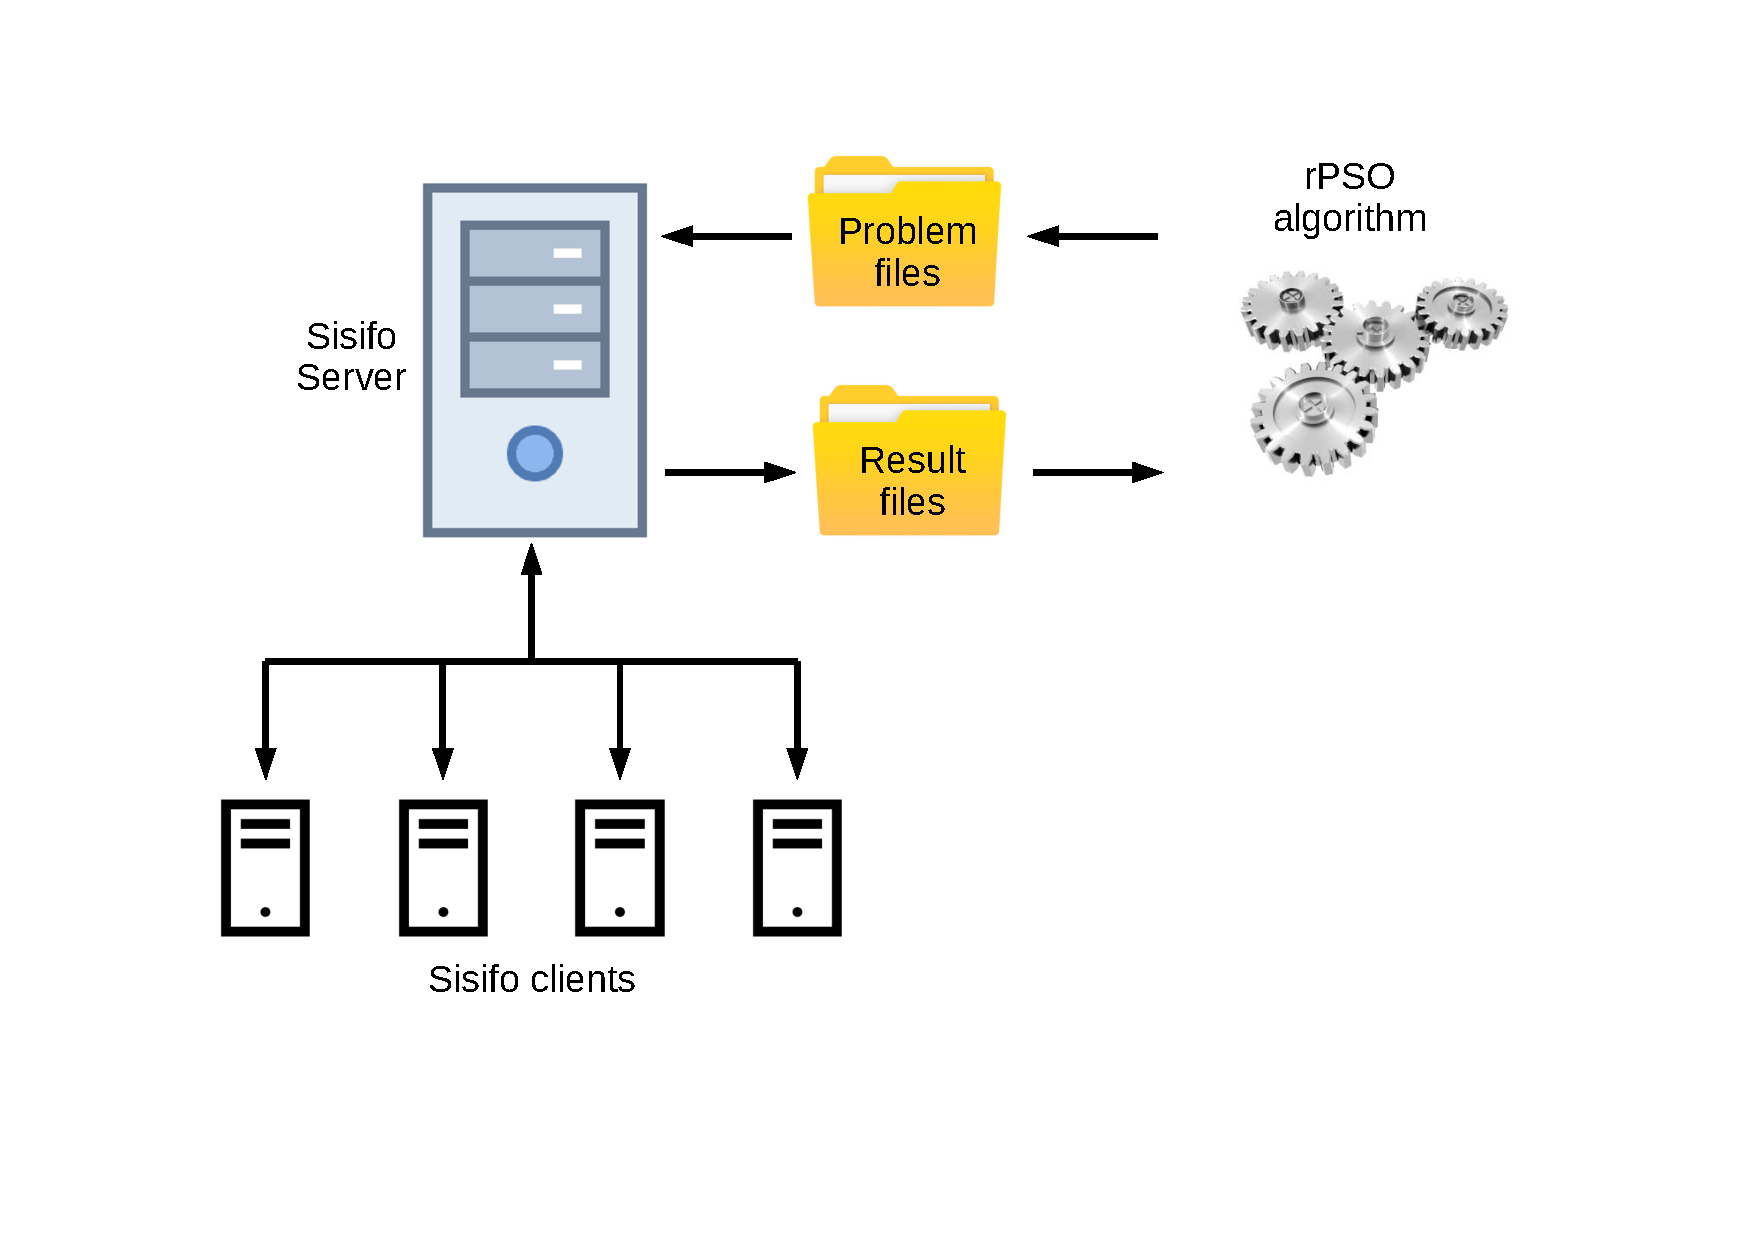
\includegraphics[width=0.6\linewidth]{IMGs/1.-Calibrado/Esquema_2.pdf}
	\caption{Introduction of the asynchronous rPSO algorithm in the Sisifo environment. rPSO manages the generation of new problems and put them in the \textit{Problem files} folder and the reading and processing of the solution files located in the \textit{Result  files} folder.}
	\label{rPSO.python}
\end{figure}

When the procedure starts running, with the initialization of the particles (Step 1) we create their corresponding problem files in the \textit{Problem files} folder. The \textit{Sisifo Server} detects new problem files and distribute them among idle \textit{Sisifo Clients}. These clients carry out the realizations. When a Sisifo client ends its task, a results file is generated and sent to the \textit{Sisifo Server} that drops it on the \textit{Result files} folder. Every time a new results file appears in the \textit{Results files} folder, the asynchronous rPSO, in Step 4, reads the data from the results file and calculates the fitness. Then, updates the velocity taking into account the current existing global best and its individual best particles (Step 2), updates the particle (Step 3) and with the new model parameters creates a new problem file in the \textit{Problem files} folder. And so on. 

\subsection{Fitness function and some features included in the rPSO}\label{sec:rPSO}
There are some features included in our version of the asynchronous rPSO algorithm that we have to describe. 

\begin{enumerate}
	\item In the Step 3, we include the possibility to discard the new particle and generate a new one randomly with $10\%$ probability. If it is not discarded, with $10\%$ probability we apply to the new particle a mutation.  
	\item The fitness evaluation is made as follows: 
	\begin{itemize}
		\item we start the model and after a warm-up time of $ 400 $ simulated months, we get a stabilization of the model output; 
		\item we take the model output from month $ 401 $ to $ 500 $ for the subpopulations in the data of Table \ref{datosConstruccion}, i.e., percentage of women HR- and LR-infected per group ages $18-29$ and $18-64$;  
		\item then, for each subpopulation, we calculate the maximum and the minimum of these portions of the model output and we see if these maximum and minimum are inside the corresponding data $95\%$ confidence interval;
		\item if this happens, the fitness is zero; 
		\item otherwise, the fitness is the sum of the distances from these maxima and minima to the corresponding $95\%$ confidence interval of the data.
	\end{itemize}
	
	\item The definition of the fitness function may provide the same fitness values for different particles. Therefore, we are going to store all the particles with the same best fitness and, in Step 2, we chose  $p_{global}^{best}$ randomly among the stored particles.	
	\item As we mentioned before, physicians around the world have published estimations of most of the model parameters \cite{Durex2002,elbasha2007model,Giuliano2011,Nyitray2015}. It is clear that we have to respect their estimation in our fitting procedure avoiding that some model parameters overpass the estimation intervals. Furthermore, finding model parameters in the range of the estimations, gives credibility to our model. Therefore, when a model parameter is less than $1\%$ closer to an extreme of the interval provided by the physician estimations, we discard this value and it is substituted by a random value inside the interval.  
\end{enumerate}

It is worth to note that the above points 1, 3 and 4 will allow us to explore extensively the whole space of parameters avoiding the accumulation of particles close to the borders. 

\begin{remark}\label{mo}
At this point, we want to remark that to evaluate the fitness function, we do not need the model output for all the subpopulations. Only is necessary the output corresponding to HR- and LR-infected women in the group ages $18-29$ and $18-64$. Then, when a realization is carried out, we retrieve and process from the results file the data corresponding to the above subpopulations from the month $401$ to $500$, write them in a row and this row is stored as the result of the realization to be used later. 

Also, in order to compare properly the model output row with the data, we build the data vector mean, percentile $2.5$ and percentile $97.5$, repeating $100$ times the $4$ values of each we have in the Table \ref{datosConstruccion} and write them in a row.
\end{remark}

\section{Selecting an optimal number of particles to calibrate the HPV large network computational model with rPSO}
As we have mentioned above, on previous implementations of the parallel rPSO, we realized that we can not affirm that \textit{the higher the number of particles, the better the quality of the solution}. Moreover, we also detected that, due to our asynchronous parallel implementation, sometimes the use of more processors does not mean lower execution times. We would need more experiments to detect the correct cause of the delays. However, in this case is more practical to investigate what the optimal combination of particles is to achieve the best quality with the lowest number of processors.

To perform this test, we are going to build HPV network models with $50,000$ nodes. We run 5 repetitions of the same problem with different number of particles. Times are shown in seconds. Thus, the question is, what is the quality of the solutions for different number of particles? Table \ref{tab.color} shows relevant information regarding the quality of the solutions for different number of particles and 5 runs of each configuration. Each run carried out 1200 particle evaluations. We measure the quality of the solutions on Table \ref{tab.color} by counting the number of fitness values equal to zero in the 5 runs (\textit{Total \# 0s}) and on average (\textit{Avg \#0s}). In addition, we also recorded the iteration at which the first zero appear on average (\textit{Avg  First}), from the last population of particles Fitness of the best, worst and average, averaged over five runs (\textit{Best at end}, \textit{Worst at end} and \textit{Avg at end}). And regarding executions time we show on Table  \ref{tab.color} information about the average total execution time for 1200 evaluations (\textit{Total Time}), the  worst execution time for one particle (\textit{Worst $t$}) and the best execution time for one particle (\textit{Best $t$}). Red color indicates the worst configuration, bold letters indicate the best and blue color the second best configuration.

\begin{table}[h]
	\centering
	\tiny \begin{tabular}{cccccccccc}
		\hline
		\cellcolor[HTML]{C0C0C0}\#       & Total   & Avg   & Avg     & Best    & Worst   & Avg  & Total   &       &                            \\
		\cellcolor[HTML]{C0C0C0} Part. &     \#0s & \#0s   &First  &  at end  & at end &at end & Time & Worst t  &          Best t                     \\ 
		\hline
		\cellcolor[HTML]{C0C0C0}25          & 18            & {\color[HTML]{3166FF} 3.60} & \textbf{531.00}                & \textbf{0.015486}               & \textbf{0.429090}               & \textbf{0.122573}               & 8422.00                         & \textbf{148.60}                & \textbf{107.00}               \\
		\cellcolor[HTML]{C0C0C0}30          & \textbf{28}           & \textbf{5.60}               & {\color[HTML]{3166FF} 594.00}  & {\color[HTML]{3166FF} 0.003785} & {\color[HTML]{3166FF} 0.445587} & {\color[HTML]{3166FF} 0.131193} & \textbf{6908.00}                & {\color[HTML]{3166FF} 186.60}  & {\color[HTML]{3166FF} 112.00} \\
		\cellcolor[HTML]{C0C0C0}35          & 8             & 1.60                        & 834.80                         & 0.010211                        & 0.576688                        & 0.149215                        & {\color[HTML]{3166FF} 7105.00}  & 250.60                         & 119.60                        \\
		\cellcolor[HTML]{C0C0C0}40          & 16            & 3.20                        & 692.80                         & 0.003332                        & 0.524417                        & 0.132628                        & 8808.60                         & 389.40                         & 144.60                        \\
		\cellcolor[HTML]{C0C0C0}45          & 14            & 2.80                        & 790.40                         & 0.006458                        & 0.639775                        & {\color[HTML]{FE0000} 0.149670} & 10004.00                        & 502.00                         & 177.20                        \\
		\cellcolor[HTML]{C0C0C0}50          & 11            & 2.20                        & 796.00                         & {\color[HTML]{FE0000} 0.005168} & {\color[HTML]{FE0000} 0.658020} & 0.139089                        & 11124.40                        & 648.40                         & 220.00                        \\
		\cellcolor[HTML]{C0C0C0}55          & 2             & {\color[HTML]{FE0000} 0.40} & {\color[HTML]{FE0000} 1171.20} & 0.004330                        & 0.518894                        & 0.137088                        & 11905.80                        & 775.00                         & 207.40                        \\
		\cellcolor[HTML]{C0C0C0}60          & 12            & 2.40                        & 765.00                         & 0.002153                        & 0.546259                        & 0.132464                        & 13787.80                        & 857.00                         & 245.40                        \\
		\cellcolor[HTML]{C0C0C0}64          & 5             & 1.00                        & 985.40                         & 0.002763                        & 0.551228                        & 0.140977                        & {\color[HTML]{FE0000} 18770.00} & {\color[HTML]{FE0000} 1041.20} & {\color[HTML]{FE0000} 379.20} \\ \hline
	\end{tabular}
	\caption{Analysis of the quality and execution times of different rPSO configurations. Results of 1200 evaluations for different number of particles on the rPSO process (\# Part.).}
	\label{tab.color}
\end{table}

As we can see, 25 and 30 particles are the preferred configurations, since we obtained the higher number of zeros in total and on average and the lower executions times. Since the results of 25 particles shows a very good run with 7 zeros and also a very good execution time, we can conclude that the configuration with 30 particles should be selected bearing in mind both quality and execution time. Results on total number of 0s and total time were statically significant with $p$ value of $0.1$ after an ANOVA analysis.

\section{Improving the exploration of the rPSO}
As we explained on Section \ref{sec:rPSO}, we established a procedure respect to the intervals for the parameter values proposed by physicians. Some algorithms such as differential evolution \cite{storn1997differential} allows to overpass these limits in the search of a good combination of parameters. However, this is not a good idea when implementing our parallel rPSO. First, remember that our parallel version is asynchronous and the updating of the particles is made once every particle is evaluated. Allowing particles with parameters close to the limits trespass them, could lead to a chaotic search. Second, parameters out the defined bounds have not a medical meaning. Therefore, when a model parameter is less than $1\%$ closer to an extreme of the interval provided by the  estimations, we discard this value and it is substituted by a random value inside the interval. This allows also to made a deeper and more efficient exploration of the search space.

Figures in Table \ref{Ctg} show the exploration performed in some of the parameters of the model (duration and contagion parameters). Figures represent the values of the parameters during the 20 executions of rPSO algorithm with 500 realizations each one. X axis represents the realization number and Y axis the value of each parameter. We can see that we find points on most of the search space.

\begin{figure}[!h]
\begin{center}	
\begin{tabular}{cc}
	Time of clearance of        & Time of clearance of \\
	HPV high risk               & HPV low risk          \\
	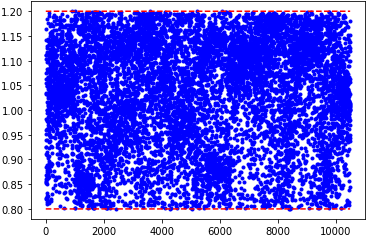
\includegraphics[width=0.45\textwidth]{IMGs/1.-Calibrado/Dura_HR_H.png} & 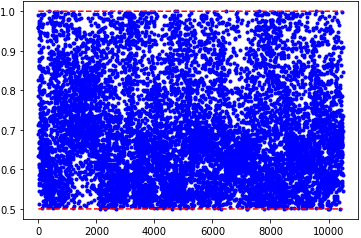
\includegraphics[width=0.45\textwidth]{IMGs/1.-Calibrado/Dura_LR_H.png} \\ 
	\\
	Women transmission probability & Men transmission probability \\
	of HPV low risk                & of HPV high risk             \\
	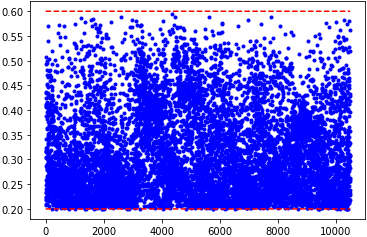
\includegraphics[width=0.45\textwidth]{IMGs/1.-Calibrado/Ctg_M_LR.png} & 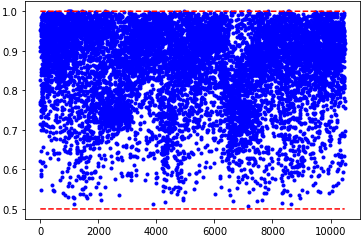
\includegraphics[width=0.45\textwidth]{IMGs/1.-Calibrado/Ctg_H_HR.png}  
\end{tabular}
\caption{Upper figures: Time of clearance of HPV high risk and low risk, both for men and women. Lower figures: on the left, probability to transmit low risk HPV if the infected is a woman; on the right, probability to transmit high risk HPV if the infected is a man. Red dashed lines correspond to the bounds of each parameter. We can see that most of the search space is explored in all the cases.} 
\label{Ctg}
\end{center}
\end{figure}

\section{Calibrating the model}
Now, we are going to perform the calibration. We use the Sisifo environment with the modified rPSO and 30 particles. The HPV network models will have $100,000$ nodes. In order to guarantee the reproducibility of the realizations, we are going to include in the problem files and store seeds for the generation of the random numbers during the calibration process.

We assume that, initially, data of prevalence from Table \ref{datosConstruccion} are not only for women but also for men. Then, we label women and men as infected randomly following these prevalence data. Also, we start running the realization and the first $400$ months are used as a warm-up period to stabilize the distribution of infected men and women. Thus, the goal is to calibrate the model parameters in such a way that the model output related to women HR and LR prevalence minimize the fitting function defined in Section \ref{sec:rPSO}.

We have performed 20 different calibrations using rPSO, each one with around $500$ realizations and $30$ particles. A total of $10,100$ realizations of the model were performed with an equivalent sequential total computation time of $161$ days.

\begin{figure}[h!]
	\centering
	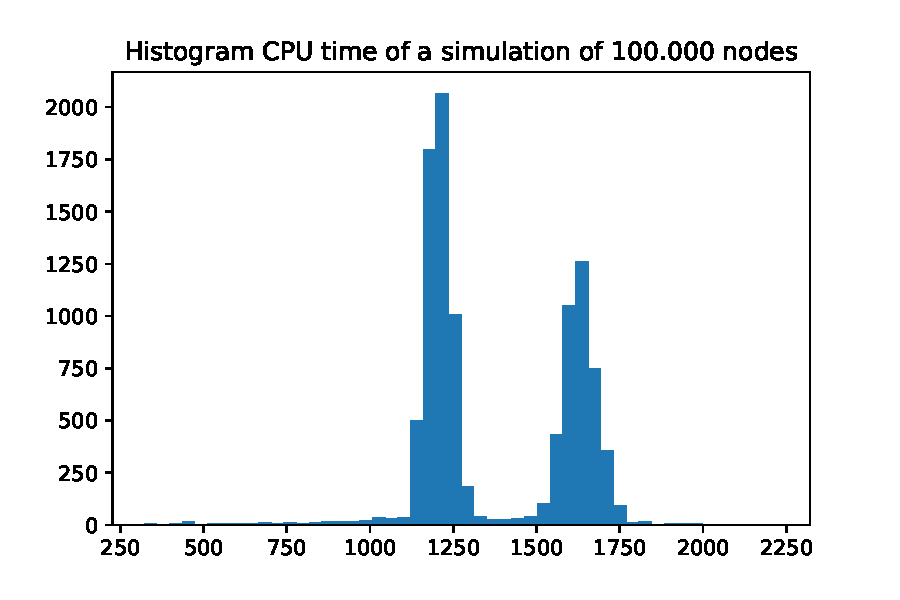
\includegraphics[width=0.6\linewidth]{IMGs/1.-Calibrado/Hist_CPU_time.pdf}
	\caption{Histogram of the computation time of each one of the $10,100$ realizations of the model using networks of $100,000$ nodes. The average time is $1374.5$ seconds, around $23$ minutes.}
\end{figure}

\section{Selecting the 30 realizations that best capture the data uncertainty}
Our goal, now, is to find a procedure to select $30$ among the $10,100$ realizations of the model in such a way that the means and the 95\% confidence intervals of these $30$ realizations be as much close as possible of the corresponding means and the 95\% confidence intervals of the data in Table \ref{datosConstruccion}. We decided to select $30$ because as we saw in Table \ref{tab.color}, the total computation time is the best for $30$ particles running in parallel in the Sandy Bridge computer.

Nevertheless, it would be interesting to reduce the number of eligible realizations to much less than $10,100$. In Figure \ref{Error_0} we can see the $100$ realizations with error less than $0.01$, that is, the realizations that almost lie inside the 95\% confidence intervals of the data, represented by the blue horizontal dashed lines. If we select $30$ among these $100$, it is clear that some percentiles of the model will be far from the corresponding percentiles of the data, for instance, the lower parts of the left figures. Therefore, we need to consider realizations with errors greater than $0.01$ without forgetting the objective to reduce the number of eligible realizations.  

\begin{figure}[h!]
	\centering
	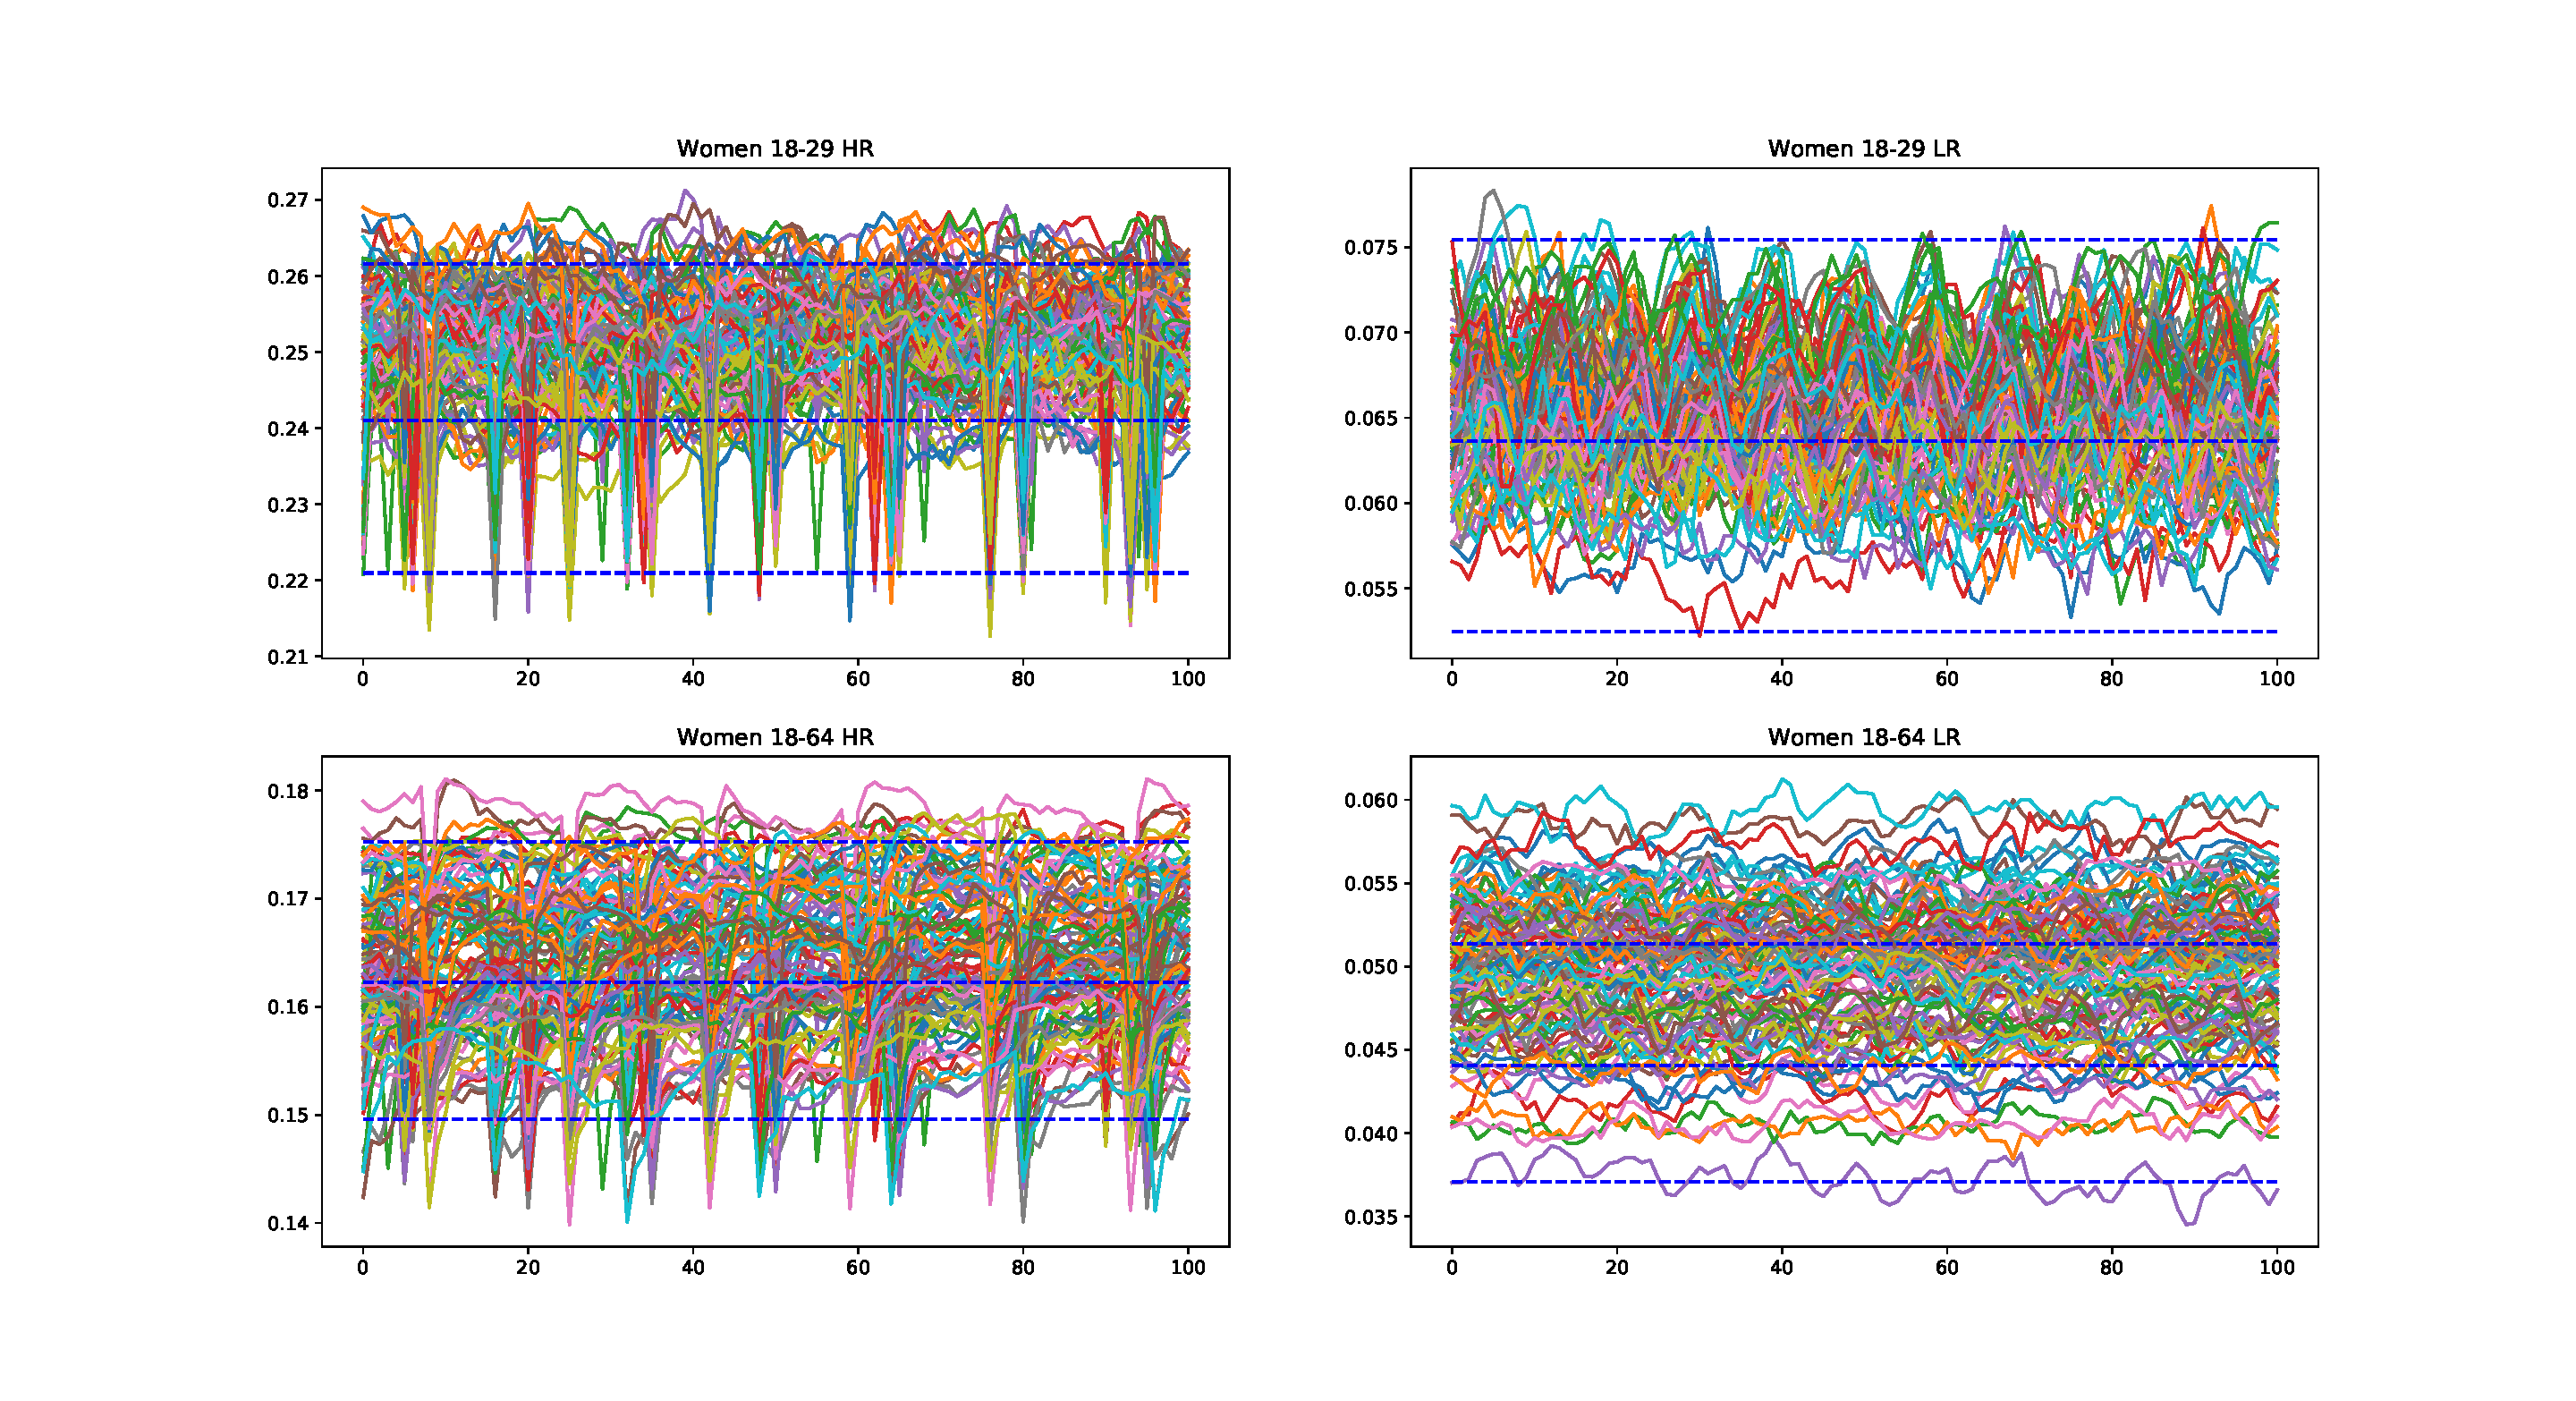
\includegraphics[width=\linewidth]{IMGs/1.-Calibrado/Error_001.pdf}
	\caption{Drawing of the $100$ model realizations with error less than $0.01$ from month 400 to 499. }
	\label{Error_0}
\end{figure}

Thus, we check the number of possible realizations depending on their error. Then, there are $2$ realizations with error $0$,  $100$ realizations with error less than $0.01$, $392$ with error less than $0.025$, $1282$ with error less than $0.05$ and $2607$ with error less than $0.075$. 
In Figure \ref{Error_003}, we draw the $1282$ model realizations of with error less than $0.05$. Note that the realizations cover completely the 95\% confidence intervals of the data. 

\begin{figure}[h!]
	\centering
	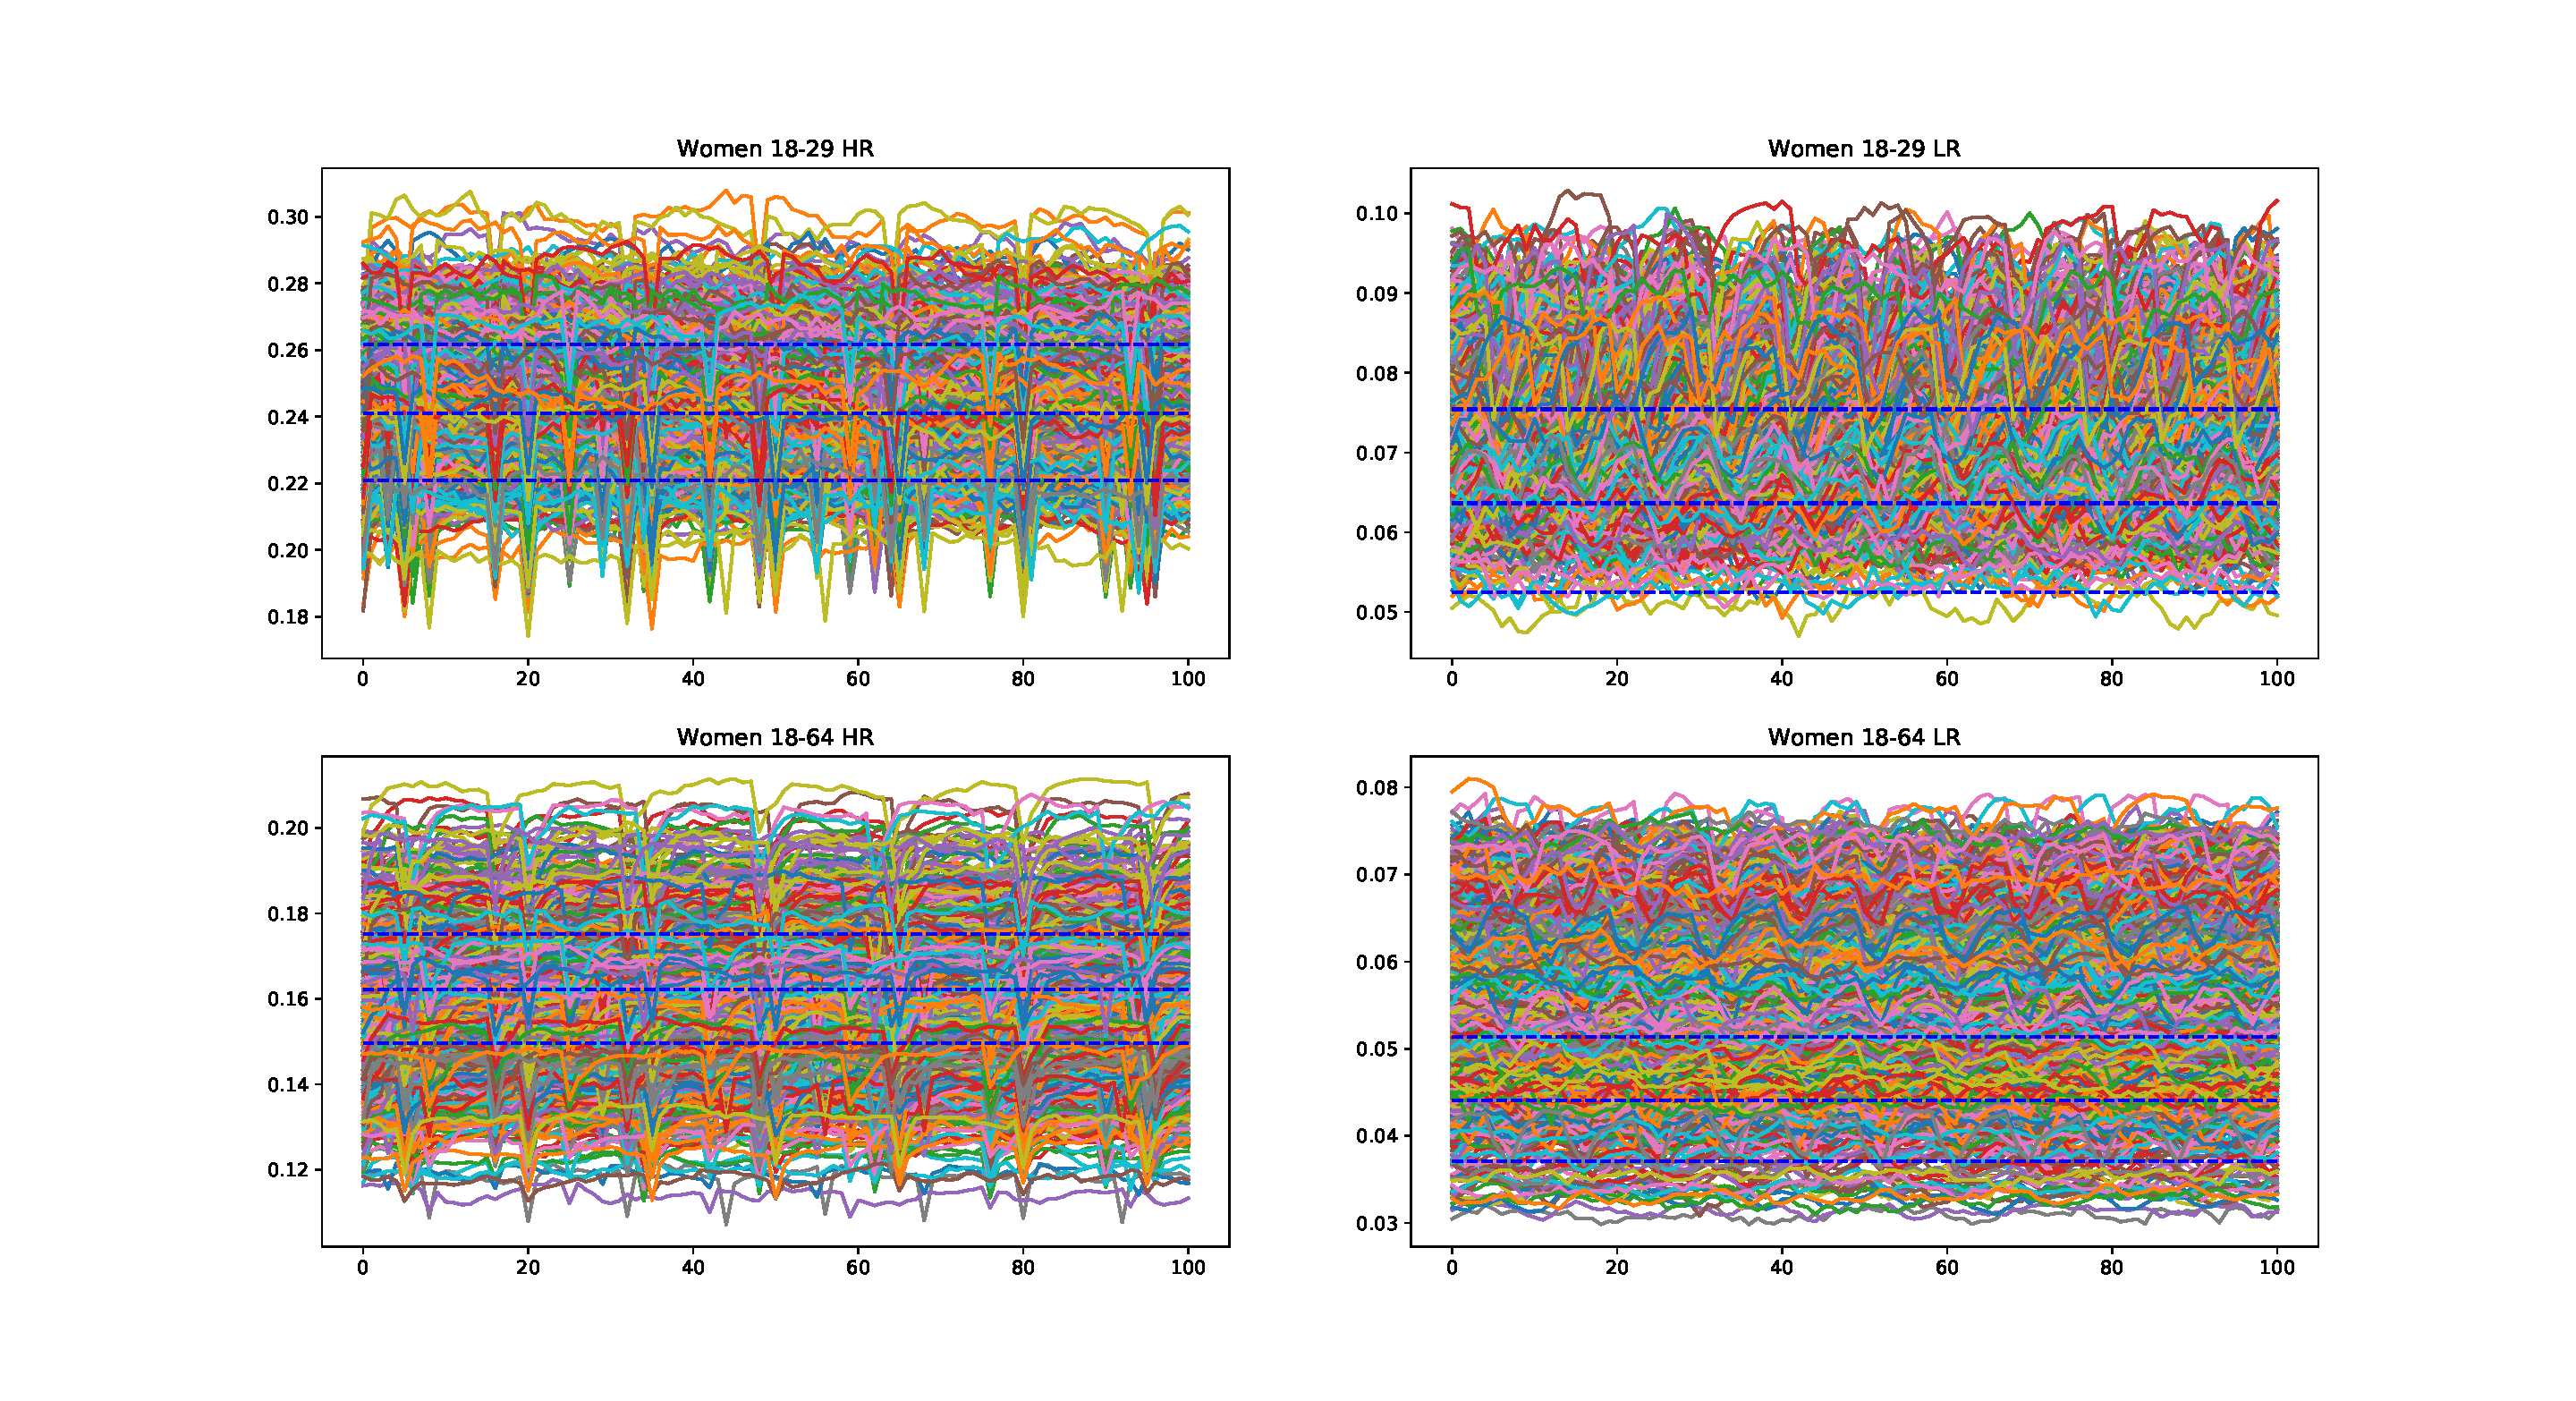
\includegraphics[width=\linewidth]{IMGs/1.-Calibrado/Error_005.pdf}
	\caption{Drawing of the $1282$ model realizations with error less than $0.05$ from month 400 to 499. These realizations cover the 95\% confidence intervals of the data, represented by the blue horizontal dashed lines.}
	\label{Error_003}
\end{figure}

In order to determine the \textit{best} $30$ realizations that capture the mean and the $95\%$ confidence intervals of the data in Table \ref{datosConstruccion}, we are going to introduce an adapted version of the rPSO algorithm before. Let $E$ be the realizations considered with $card(E)=M$ its number. For instance, for $E$ the set of realizations with error less than $0.01$, $M=100$. Also, for $E$ the set of realizations with error less that $0.05$, $M=1282$. Then $E(i)$ is the $i-th$ realization of the set $E$. We define the following fitness function $F$:

\begin{description}
	\item[INPUT:] Set of $30$ indexes $I=\{i_1,\ldots,i_{30} \}$, $1\leq i_j \leq M$, $j=1,\ldots, 30$..
	\item[Step 1.] Select the realizations $E(i_1),\ldots,E(i_{30})$ and calculate the mean, percentile $2.5$ and percentile $97.5$ of them.
	\item[Step 2.] Calculate the norm of the difference between the mean, percentile $2.5$ and percentile $97.5$  of the $30$ realizations and the data (see Remark \ref{mo}), and sum them up. 
\end{description}

Now, the adapted version of rPSO to select the best $30$ realizations is

\begin{description}
	\item[Step 1.] Initialization.
	\begin{itemize}
		\item We have a set $E$ with $M$ realizations.
		\item Initialize $N$ index subsets $S_1,\ldots,S_N$ with $30$ elements of the set $\{1,\ldots,M\}$ (particles) chosen randomly without repetition.
		\item Evaluate the fitness of all the particles $F(S_1), \ldots, F(S_N)$.
		\item Define the individual best fitness as $S_i^{best} = S_i$, $i=1,\ldots,N$ and the global best fitness $S_{global}^{best}$ as the $S_i^{best}$ which fitness is the minimum.
	\end{itemize}
	\item[Step 2.] For $i=1,\ldots,N$, build the new set $P_i=S_i \cup S_i^{best} \cup S_{global}$, that is, joining the current particle, its individual best and the global best. After removing index repetitions, the new particle $S_i$ consists of a random selection without repetition of $30$ indexes of $P_i$.
	\item[Step 3.] Evaluate the fitness of all the new particles $F(S_1), \ldots, F(S_N)$.	
	\item[Step 4.] Update the individual best fitnesses $S_i^{best} = p_i$, $i=1,\ldots,N$ and  the global best fitness $S_{global}^{best}$. Go to Step 2. 
\end{description}

Here, we also consider $10\%$ of randomness and $10\%$ of mutation when updating new particles. In this case, mutation consists of changing some of the indexes in the current particle by other randomly chosen indexes, avoiding repetitions.

The above algorithm, in the tests we have run, lasts around $20$ minutes for $1$ million of evaluations of the fitness function in the Sandy Bridge computer, returning accurate solutions.

We have performed runs for $30$, $40$, $50$ and $60$ particles, being $E$ the realization sets with errors less than $0.025$, $0.05$ and $0.075$. The lowest error has been $0.1166$ for the following realizations  

\begin{equation}
\begin{array}{c}
85, 109, 460, 474, 475, 476, 485, 493, 496, 497, 523, 531, \\
542, 543, 563, 600, 635, 637, 650, 687, 715, 729, 730, \\
842, 974, 987, 1058, 1060, 1080, 1238,	
\end{array}
\label{laselegidas}    
\end{equation}

among the $1282$ of the set of realizations with error less than $0.05$. In Figure \ref{fig:laselegidas} we draw the selected realizations and in Figure \ref{fig:ajuste95IC} we can see the graphical result of the calibration and how resemble the means and 95\% confidence intervals.  

\begin{figure}[h!]
	\centering
	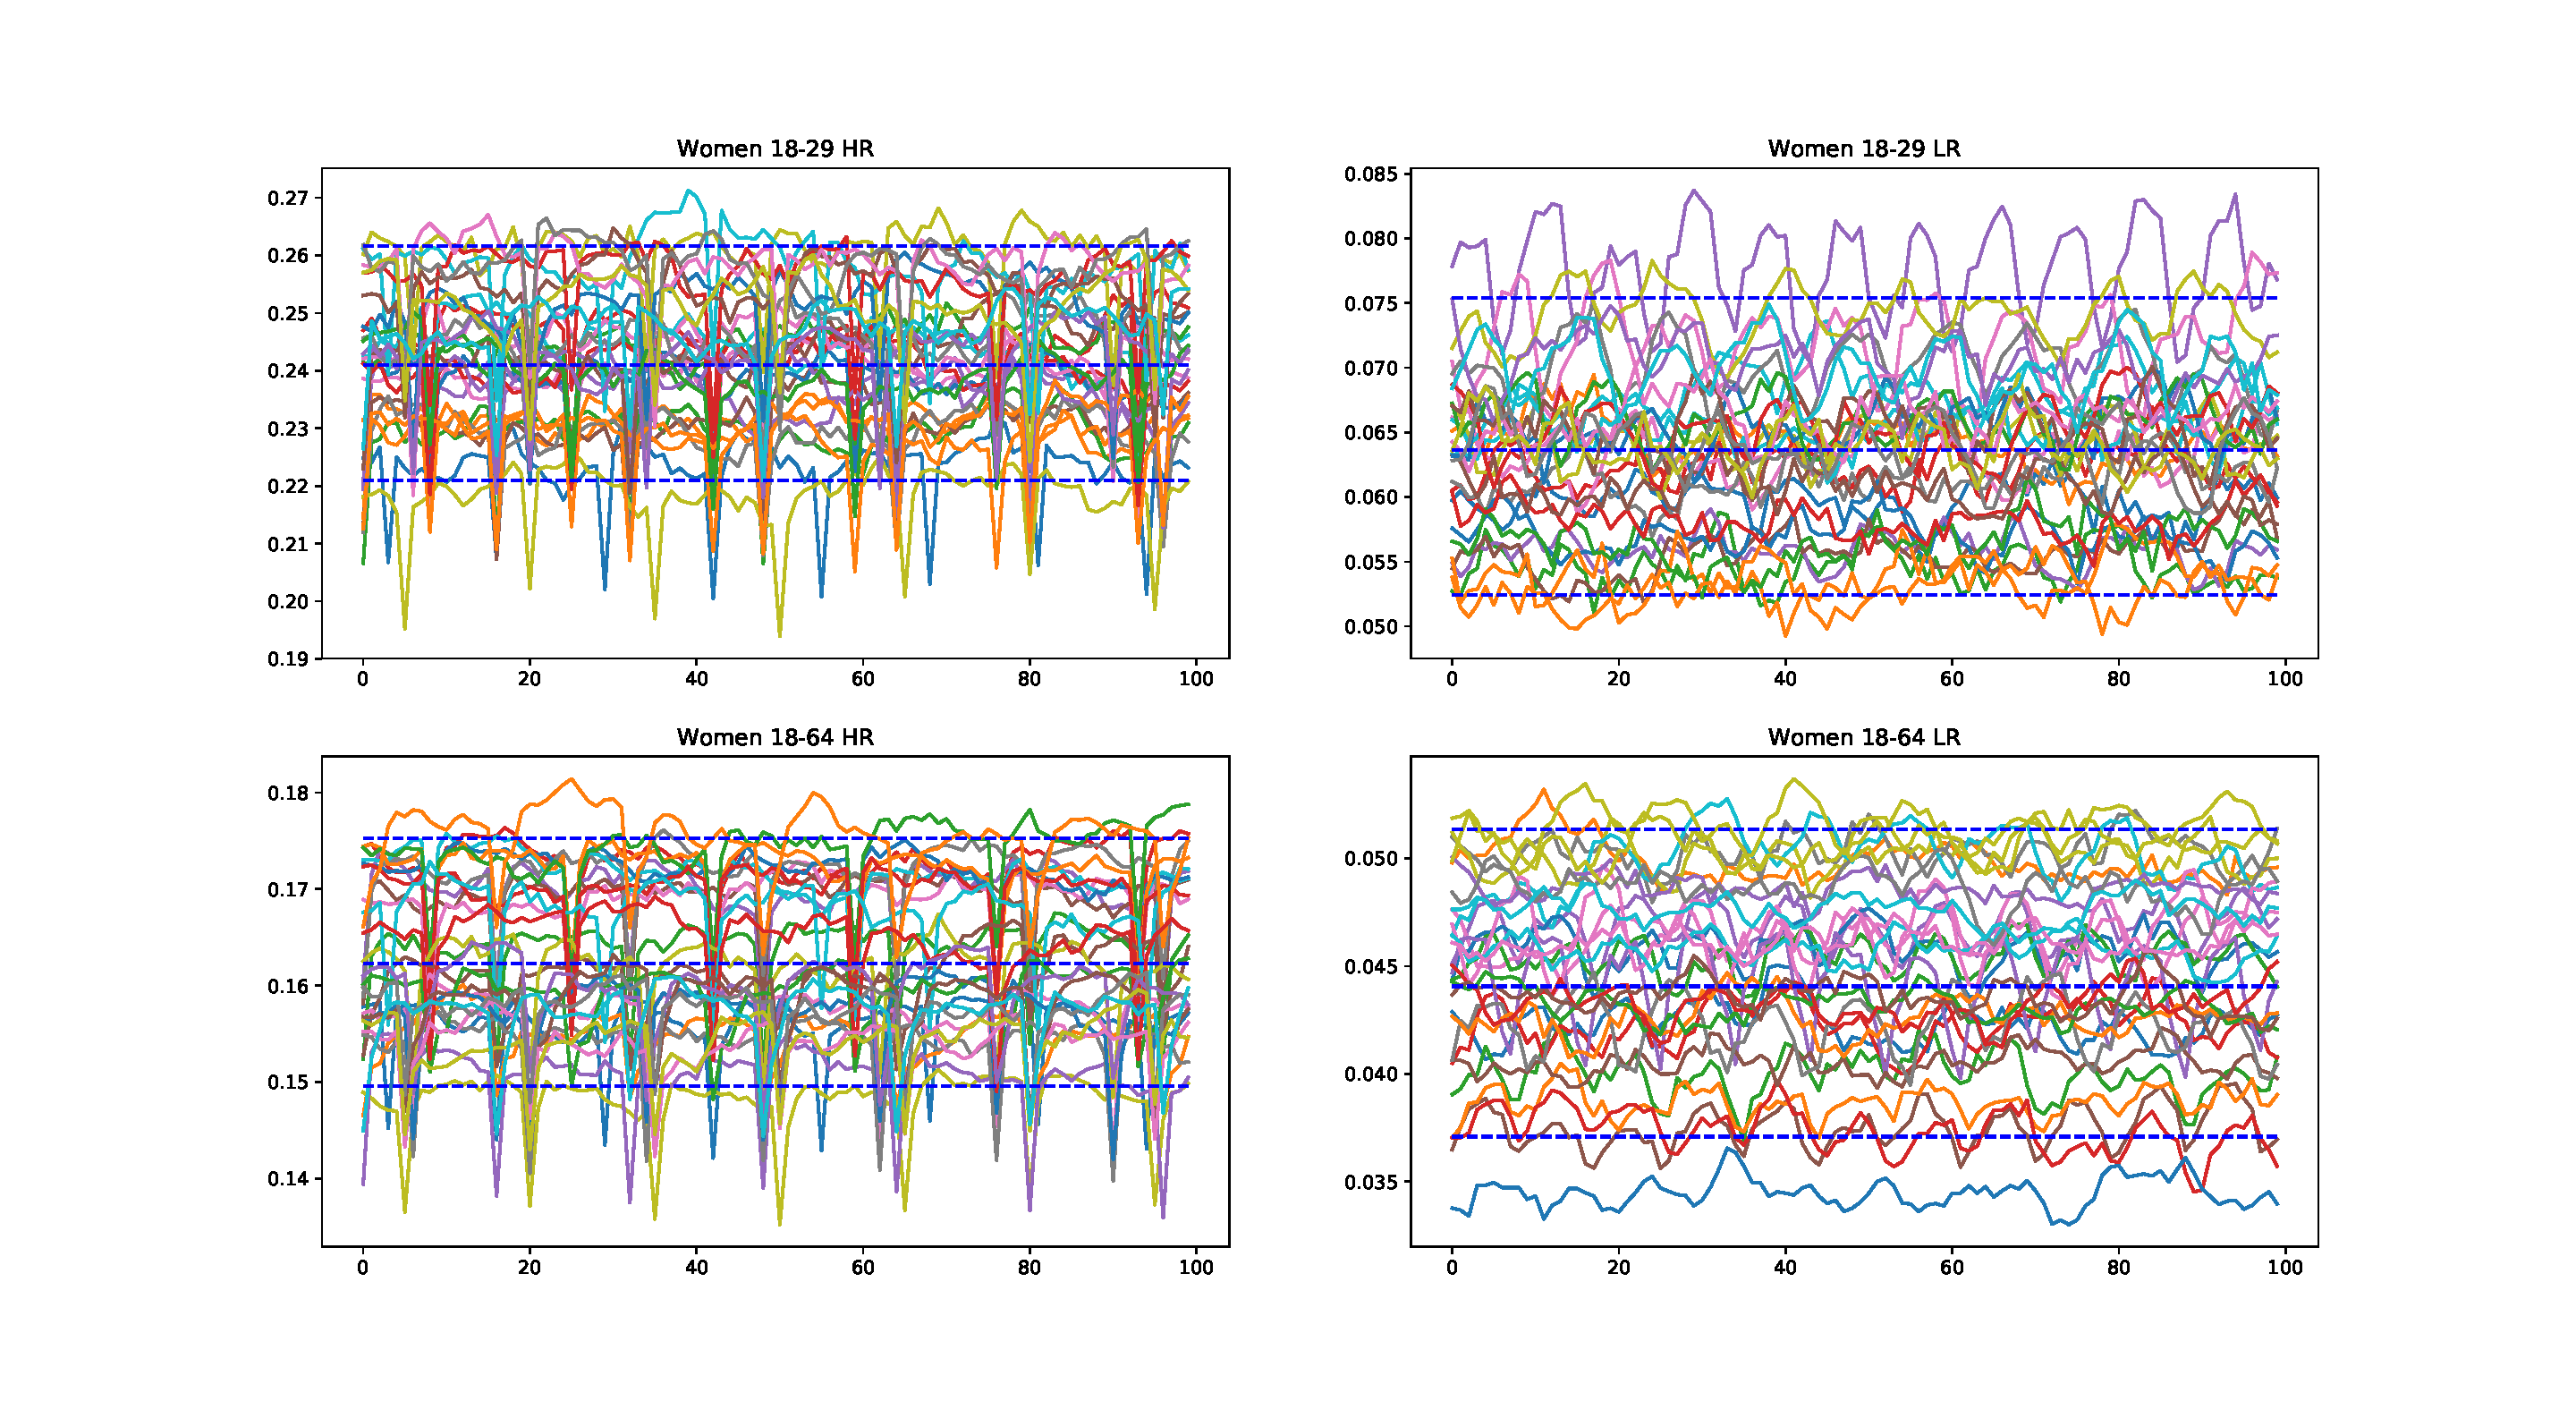
\includegraphics[width=\linewidth]{IMGs/1.-Calibrado/Selected.pdf}
	\caption{Drawing of the $30$ selected model realizations from month 400 to 499. These realizations are the ones whose means and 95\% confidence intervals resemble the most the data in Table \ref{datosConstruccion}, represented by the blue horizontal dashed lines.}
	\label{fig:laselegidas}
\end{figure}

\begin{figure}[h!]
	\centering
	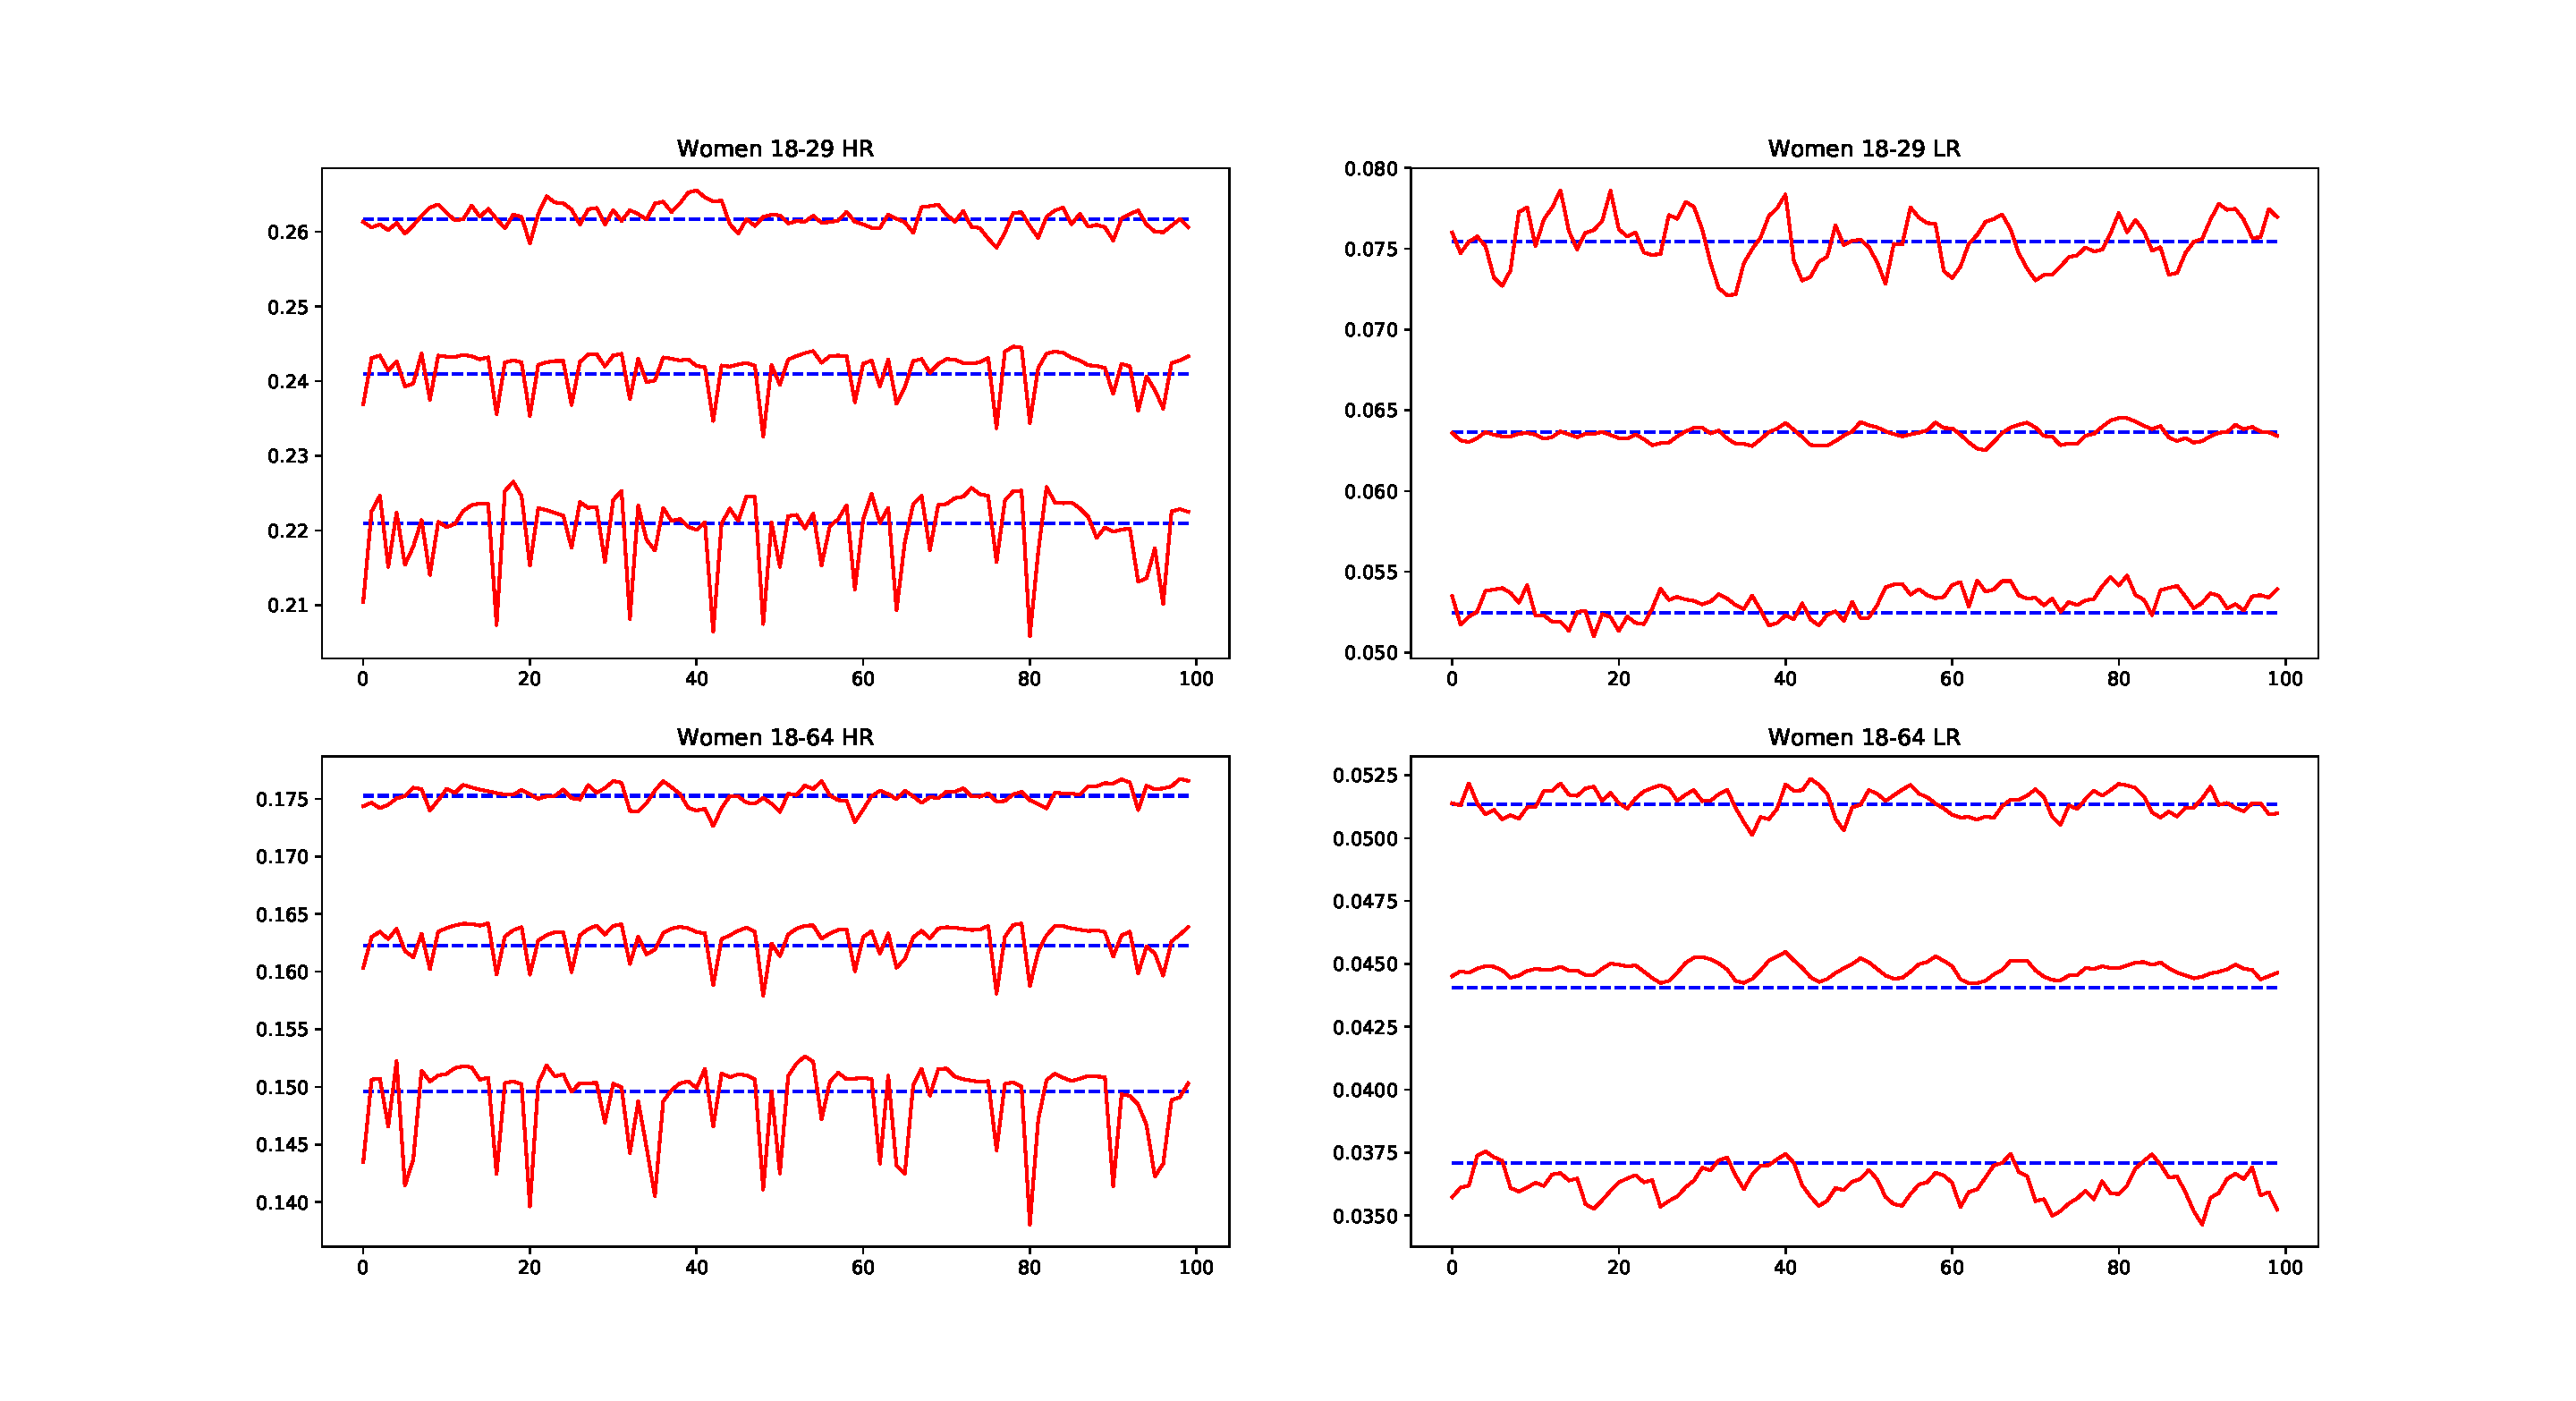
\includegraphics[width=\linewidth]{IMGs/1.-Calibrado/Ajuste_95IC.pdf}
	\caption{Means and 95\% confidence intervals of the $30$ selected realizations (in red) compared to the means and 95\% confidence intervals of the data (blue).}
	\label{fig:ajuste95IC}
\end{figure}

The mean and the 95\% confidence interval of the model parameters corresponding to the $30$ selected realizations from \eqref{laselegidas} are given in the Table \ref{table:laselegidas}. Note that the obtained model parameters are in accordance to the medical parameters appearing in the literature and collected in Section \ref{sec:modelo}. 

\begin{table}[!h]
	\begin{center}
		\begin{tabular}{|c|c|c|}
			\hline 
			Model parameter & Mean & $95\%$ confidence interval  \\ 
			\hline 
			Average LSP men & $8.63$ & $ [ 7.15 ,  9.86 ]$  \\ 
			Average time clearing HR HPV & $1.08$ &  $[ 0.88 ,  1.19 ]$ \\ 
			Average time clearing LR HPV &  $0.60$ & $ [ 0.52 ,  0.82 ]$\\ 
			Probability a woman transmits LR &  $0.23$ &  $[ 0.21 ,  0.29 ]$\\ 
			Probability a man transmits LR &  $0.28$ &  $[ 0.22 ,  0.37 ]$\\ 
			Probability a woman transmits HR &  $0.81$ & $[ 0.68 ,  0.95 ]$\\ 
			Probability a man transmits HR &  $0.91$ & $[ 0.74 ,  0.97 ]$ \\
			\hline
		\end{tabular}
	\end{center} 	
	\caption{Mean and the 95\% confidence interval of the model parameters corresponding to the $30$ selected realizations from \eqref{laselegidas}.}
	\label{table:laselegidas}
\end{table}
%GM_hom 7.890084666666667 , [ 7.055565249999999 ,  9.175369750000002 ]
%Dura_HR_H 1.0815233666666668 , [ 0.984595275 ,  1.1799214999999998 ]
%Dura_LR_M 0.6020232666666666 , [ 0.520799475 ,  0.7130141 ]
%Ctg_M_LR 0.24630120000000003 , [ 0.20750732500000002 ,  0.29335349999999993 ]
%Ctg_H_LR 0.2989984000000001 , [ 0.227862775 ,  0.38451014999999994 ]
%Ctg_M_HR 0.7533814333333333 , [ 0.5907493 ,  0.8939666999999999 ]
%Ctg_H_HR 0.8972156666666666 , [ 0.77310225 ,  0.9853232749999998 ]

In the following, we are going to use the sets of parameters corresponding to the realizations \eqref{laselegidas} (and their corresponding seeds) to perform the simulations below. 
